\section{Probabilistic and maximum likelihood models}

For a given network \(G(V, E)\), \textbf{\emph{the probabilistic model
        optimizes an objective function to set up a model that is composed of
        several parameters}}. Observed data of the given network can be
estimated by this model nicely. At that point, the likelihood of the
presence of a non-existing link \((i, j)\) is evaluated using
conditional probability \(P(A_{i j} = 1 | \Theta )\). Several
\texttt{probabilistic\ models} and \texttt{maximum\ likelihood\ models}
have been proposed in the literature to \textbf{infer missing links in
    the networks}.\\

\textbf{The probabilistic models normally require more information like
    node or edge attribute knowledge in addition to structural information}
Extracting these attribute information is not easy; moreover, the
parameter tuning is also a big deal in such models that limit their
applicability. \emph{Maximum likelihood methods are complex and
    time-consuming}, so these models are not suitable for real large
networks.

\subsection{Local probabilistic model for link prediction}

\textbf{Wang et al.} proposed a \texttt{local\ probabilistic\ model} for
link prediction in an \emph{undirected network}. They employed three
different types of features viz., topological, semantic, and
cooccurrence probability features extracted from different sources of
information.\\

They presented an idea of a central neighborhood set derived from the
local topology of the considered node-pair, which is relevant
information for the estimation of a link between them. They computed
non-derivable frequent itemsets (i.e., those itemsets whose occurrence
statistics can not be derived from other itemset patterns) from the
network events log data, which is further used as training data for the
model. An event corresponds to a publication of a paper (i.e., authors'
interactions in the paper is a an event, and a set of such events is the
event log) in the Coauthorship network. The model is shown in the
following Figure, which considers the approach described below.\\

First, the central neighborhood set between \(x\) and \(y\) is
calculated based on local event log data. One of the usual ways to find
the central neighborhood set is to find the \textbf{shortest path
    between two vertices of specified length}, and the vertices are lying on
this path can be included in the required set. There can be more than
one shortest path between two vertices, so more neighborhood sets can be
possible. Neighborhood sets of shorter lengths and more frequent
(frequency score is used when more shortest paths of the same length are
available) are chosen for the central neighborhood set. The authors
considered the shortest path up to length 4 since the nodes lying on the
shorter length path are more relevant.\\

In the second step, for a given central neighborhood set, non-derivable
frequent itemsets are used to learn the local probabilistic model.
\textbf{Calders et al.} proposed a depth-first search method to
calculate non-derivable itemsets and the same algorithm used by the
authors. Why non-derivable frequent itemsets? \textbf{Pavlov et al.}
first introduced the concept of frequent itemset to construct an
\texttt{MRF}. They argued that a \(K-itemset\) and its support
represents a \(K-way\) statistics, which can be viewed as a constraint
on the true underlying distribution that generates the data. Given a set
of itemset constraints, a maximum entropy distribution satisfying all
these constraints is selected as the estimate for the true underlying
distribution. This maximum entropy distribution is equivalent to an
\texttt{MRF}. Since the number formed links are very few compared to all
possible links in a sparse network, the authors used a support threshold
of one to extract all frequent itemsets. Theses extracted itemsets are
large in number that results in expensive learning for the \texttt{MRF}.
To reduce this cost, only non-derivable itemsets are extracted. They
find all such itemsets that lie entirely within the central neighborhood
set. Using these itemsets, a \texttt{Markov\ Random\ Field} is
\textbf{learned}.\\

In the last step, the \texttt{iterative\ scaling\ algorithm} is used to
learn a local \texttt{MRF} for the given central neighborhood set. This
process continues overall itemset constraints and continuously updates
the model until the model converges. Once the model learning process is
over, one can infer the co-occurrence probability by computing the
marginal probability over the constructed model. The
\texttt{Junction\ tree\ inference\ algorithm} is used to infer
co-occurrence probability. The algorithm to induce co-occurrence
probability feature for a pair of vertices can be found in
\href{https://static.aminer.org/pdf/PDF/000/303/209a_parameterized_probabilistic_model_of_network_evolution_for_supervised_link.pdf}{Local
    Probabilistic Models for Link Prediction}.

\subsection{Probabilistic relational model for link prediction (PRM)}

Existing works show that \textbf{node attributes play a significant role
    to improve the link prediction accuracy}. However, \textbf{no generic
    framework is available to incorporate node and link attributes} and
hence, not applicable to all scenarios. To this end, \textbf{the
    probabilistic model is a good and concrete solution that provides a
    systematic approach to incorporate both node and link attributes in the
    link prediction framework}. Pioneering works on \texttt{PRM} include
\textbf{Getoor et al.} study on directed networks, \textbf{Taskar et
    al.} study on undirected networks, \textbf{Jennifer Neville}
work on for both networks, etc. published in \texttt{JMLR} is based on
\texttt{Relational\ Bayesian\ network\ (RBN)} where relation links are
directed and published in NIPS is based on
\texttt{Relational\ Markov\ network\ (RMN)} where relational links are
undirected.\\

\texttt{PRM} was originally designed for attribute prediction in
relational data, and it later extended to link prediction task. The
authors employed the attribute prediction framework to link prediction.
This casting can be understood with the following example: - Consider
the problem of link prediction in a coauthorship network. Non-relational
frameworks of link prediction consider only one entity type
``\emph{person}'' as node and one relationship; however, relational
framework (\texttt{PRMs}) include more entity types like article,
conference venue, institution, etc. Each entity can have attributes like
a person (attributes: name, affiliation institute, status (student,
professor)), article (attributes: publication year, type (regular,
review)), etc. Several relational links may possible among these
entities like advisor-advisee/research scholar relation between two
persons, author relationship between person and paper entities, and
paper can be related to the conference venue with publish relationship.
Moreover, relationships (links) among these entities can also have
attributes viz., exists (if there is a link between the two involved
entities), or not-exist (no link between the involved entities). This
way, the link prediction can be reduced to an attribute prediction
framework/model.\\

During the model training, a single link graph is constructed that
incorporates above heterogeneous entities and relationships among them.
Model parameters are estimated discriminatively to maximize the
probability of the link existence and other parameters with the given
graph attribute information. The learned model is then applied using
probabilistic inference to predict missing links.\\

\subsection{Hierarchical structure model (HSM)}

These models are based on the assumption that the structures of many
real networks are hierarchically organized, where nodes are divided into
groups, which are further subdivided into subgroups and so forth over
multiple scales. Some representative work systematically encodes such
structures from network data to build a model that estimates model
parameters using statistical methods. These parameters are then used in
estimating the link formation probability of unobserved links.\\

Some studies suggest that many real networks, like biochemical networks
(protein interaction networks, metabolic networks, or genetic regulatory
networks), Internet domains, etc. are hierarchically structured. In
hierarchical networks, vertices are divided into groups, which are
further sub-divided into subgroups and so forth over multiple scales.
\textbf{Clauset et al.} proposed a probabilistic model that takes a
hierarchical structure of the network into account. The model infers
hierarchical information from the network data and further applies it to
predict missing links.\\

The hierarchical structures are represented using a tree (binary), or
dendrogram, where, the leaves (i.e., \(n\) ) represent the number of
total vertices in the network and each internal vertex out of (
\(n - 1\) ) corresponds to the group of vertices descended from it. Each
internal vertex \(r\) is associated with a probability \(p_r\) , then
the existing edge probability \(p_{xy}\) between two vertices \(x\) and
\(y\) is given by \(p_{xy} = p_r\) where, \(r\) is their lowest common
ancestor. The hierarchical random graph is then, represented by the
dendrogram \(D^{\star}\) with the set of probability \(\{ p_r \}\) as
\(\left( D^{\star},\{p_r\} \right)\). Now the learning task is to find
the hierarchical random graph(s) that best estimates the observed
real-world network data. Assuming all possible dendrograms to be equally
likely, Bayes theorem says that the probability of the dendrogram
\(\left(D^{\star}, \{p_r\} \right)\) that best estimates the data is
proportional to the posterior probability or likelihood, \(L\) from
which the model generates the observed network and our goal is to
maximize \(L\) . The likelihood of a hierarchical random graph
\(\left(D^{\star},\{p_r\} \right)\) is computed using the following
equation

\[
    L(D^{\star}, \{p_r\}) = \prod_{r \in D^{\star}} p_r^{E_r} (1-p_r)^{L_r R_r - Er},
\]

where \(L_r\) and \(R_r\) are the left and right subtree rooted at
\(r\), and \(E_r\) is the number of links in the network whose endpoints
have \(r\) as their lowest common ancestor in \(D^{\star}\) . The above
equation assumes the convention \(0^0 = 1\). For a given dendrogram
\(D^{\star}\) , it is easy to compute the probability \(p_r\) that
maximizes \(L(D^{\star}, \{p_r\})\) i.e.

\[
    \overline{p_r} = \frac{E_r}{L_r R_r}.
\]

This can be understood with the following example illustrated in the
next Figure. Now, this model can be used to estimate the missing links
of the network as follows. Sample a large number of dendrograms with
probability proportional to their likelihood. Then, compute the mean
connecting probability \(\overline{p_{xy}}\) of each nonexisting pair
\((x, y)\) by averaging the corresponding probability \(p_{xy}\) overall
sampled dendrograms. Sort these vertices pairs scores in descending
order and selects top-l links to be predicted.

\begin{figure}[H]
    \centering
    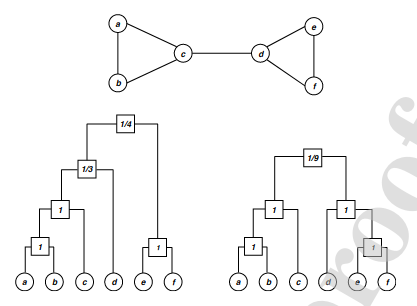
\includegraphics[width=8cm, keepaspectratio]{capitoli/methods/imgs/img8.png}
    \caption{ An illustrating example of \texttt{HSM} for a graph of 6 nodes and its
        two possible dendrograms. The internal nodes of each dendrogram are
        labeled as the maximum likelihood probability \(\overline{p}_r\). The
        likelihoods of the left and the right dendrograms are
        \(L(D1) = (1/3)(2/3)^2 (1/4)^2(3/4)^6\) \(= 0.00165\), and
        \(L(D2) = (1/9)(8/9)^8 = 0.0433\). Thus, the second (i.e., right)
        dendrogram is most probable as it divides the network in a balanced one
        at the first level.}
\end{figure}

\subsection{Stochastic block model (SMB)}

Hierarchical structures may not represent most networks. A more general
approach to represent these networks is block model where vertices are
distributed (partitioned) into blocks or communities and the connecting
probability between two vertices depends on blocks they belong to.
\textbf{Guimera et al.} presented a novel framework where stochastic
block model representation of a network is employed to find missing and
spurious links. The authors compute the reliability of the existence of
links given an observed network that is further used to find missing
links (non-existing links with higher reliabilities) and spurious links
(existing links with lower probabilities).\\

The link reliability \(R_{xy}\) between the two vertices \(x\) and \(y\)
is

\[R_{xy} = p_{BM} (A_{xy} = 1 | A^0).\]

i.e.~probability that the link truly exists given the observed network
\(A^0\), the block model \(BM\).\\

Generally, complex networks are outcomes of combination of mechanisms,
including modularity, role structure, and other factors. In \(SBM\),
partitioning vertices of network based on these mechanisms may result in
different block models that capture different correlations (patterns) of
the network. Assume that no prior knowledge of suitable models, the
reliability is expressed as

\[
    R_{xy} = \frac{1}{Z} \sum_{P \in P^{\star}} \left( \frac{l^{0}_{\sigma_x \sigma_y} + 1}{r^{0}_{\sigma_x \sigma_y + 2}} \right) \text{ exp } \left[ -H(P) \right],
\]

where the sum is over all possible partitions \(P^{\star}\) of the
network into groups, \(\sigma_x\) and \(\sigma_y\) are vertices \(x\)
and \(y\) groups in partition \(P\) respectively. Moreover, \(l^0_1\)
and \(r^0_{\sigma_{\alpha} \sigma_{\beta}}\) are the number of links and
maximum possible links in the observed network between groups \(\alpha\)
and \(\beta\) . The function \(H(P)\) is

\[H(P) = \sum_{\alpha \leq \beta} \left[ \ln \left( r_{\alpha \beta} \right) + \ln \binom {r_{\alpha \beta}}{l^0_{\alpha \beta}} \right],\]

and \(Z = \sum_{P \in P^{\star}} \text{ exp } \left[ -H(P) \right]\).\\

Practically, solving equation \(R_{xy} = \ldots\) , i.e., summing over
all possible partitions is too complex even for a small network.
However, the Metropolis algorithm can be used to correctly sample the
relevant partitions and obtain link reliability estimates.\\

The authors employed the link reliability concept to find missing links
and to identify the spurious link in the networks with the following
procedure.

\begin{itemize}
    \item
          \((i)\) Generate the observed network \(A^0\) by removing/adding some
          random links (for finding missing/spurious links) from/to the true
          network \(A^t\) .
    \item
          \((ii)\) Compute the link reliability for non-observed links (i.e.
          non-existing \(+\) missing/spurious links).
    \item
          \((iii)\) Arrange these links with their reliability score in
          decreasing order and decide the top-l links as desired ones (i.e.,
          missing/spurious links).
\end{itemize}

Probabilistic and maximum likelihood methods extract useful features and
valuable correlation among the data using hierarchical and stochastic
block models, which result in significant improvements in prediction
results as compared to some similarity-based methods. However, these are
\textbf{quite complex and time-consuming even on small datasets} that
limit their applicability on large scale real-world network datasets.

\subsection{Exponential random graph model (ERGM) or P-star model}
